The adjoining figure shows two intersecting chords in a circle, with $B$ on minor arc $AD$.  Suppose that the radius of the circle is 5, that $BC = 6$, and that $AD$ is bisected by $BC$.  Suppose further that $AD$ is the only chord starting at $A$ which is bisected by $BC$.  It follows that the sine of the minor arc $AB$ is a rational number.  If this fraction is expressed as a fraction $m/n$ in lowest terms, what is the product $mn$?
\begin{center}
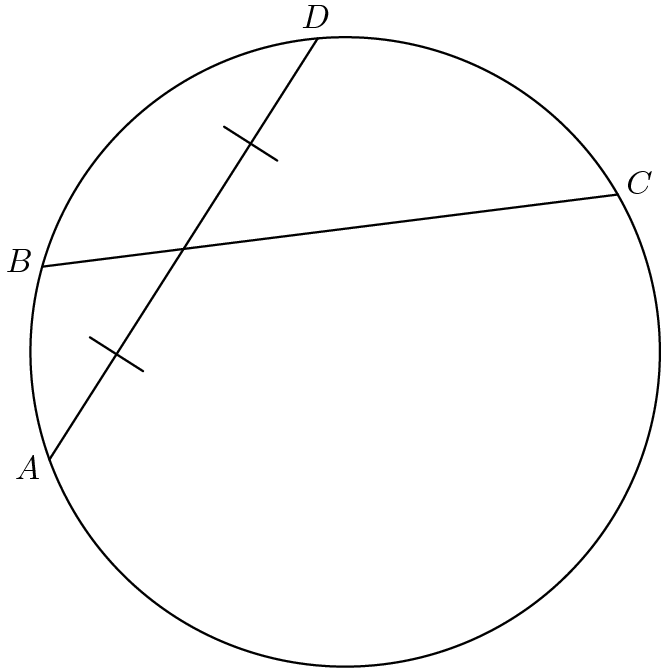
\includegraphics[width = 66.4mm]{img/fig0.png}
\end{center}